\documentclass{article}

% if you need to pass options to natbib, use, e.g.:
     \PassOptionsToPackage{numbers, compress}{natbib}
% before loading neurips_2019

% ready for submission
% \usepackage{neurips_2019}

% to compile a preprint version, e.g., for submission to arXiv, add add the
% [preprint] option:
    \usepackage[preprint]{neurips_2019}

% to compile a camera-ready version, add the [final] option, e.g.:
%     \usepackage[final]{neurips_2019}

% to avoid loading the natbib package, add option nonatbib:
%     \usepackage[nonatbib]{neurips_2019}

\usepackage[utf8]{inputenc} % allow utf-8 input
\usepackage[T1]{fontenc}    % use 8-bit T1 fonts
\usepackage{hyperref}       % hyperlinks
\usepackage{url}            % simple URL typesetting
\usepackage{booktabs}       % professional-quality tables
\usepackage{amsfonts}       % blackboard math symbols
\usepackage{nicefrac}       % compact symbols for 1/2, etc.
\usepackage{microtype}      % microtypography
\usepackage{listings}       % for code listings
\usepackage{graphicx}       % for images
%\usepackage{inconsolata}   % use as code font
\usepackage{color}          % for custom colors
\usepackage{lipsum}

% Define custom colors
\definecolor{deepblue}{rgb}{0,0,0.5}
\definecolor{deepred}{rgb}{0.6,0,0}
\definecolor{deepgreen}{rgb}{0,0.5,0}
\definecolor{gray}{rgb}{0.3,0.3,0.3}

% Some settings for code
\lstset{
    basicstyle=\small\ttfamily, 
    breaklines=true,
 %   frame=lines,
    showstringspaces=false,
    tabsize=1,
    breakatwhitespace=false,
    stringstyle=\color{deepgreen},
    keywordstyle=\bfseries\color{deepblue},
    commentstyle=\color{gray},
    emphstyle=\color{deepred},
    emph={spells,spellbook,geomancer,tests,conftest},
}


\title{Geomancer: An Open-Source Framework for Geospatial Feature Engineering}

% The \author macro works with any number of authors. There are two commands
% used to separate the names and addresses of multiple authors: \And and \AND.
%
% Using \And between authors leaves it to LaTeX to determine where to break the
% lines. Using \AND forces a line break at that point. So, if LaTeX puts 3 of 4
% authors names on the first line, and the last on the second line, try using
% \AND instead of \And before the third author name.

\author{%
  \textbf{Lester James V. Miranda, Mark Steve Samson, Alfiero K. Orden II}\\
  \textbf{Bianca S. Silmaro, Ram K. De Guzman III, Stephanie S. Sy}\\
  Thinking Machines Data Science\\
  Metro Manila, Philippines\\
  \texttt{\{lj,marksteve,ardie,bianca,ram,stef\}@thinkingmachin.es} \\
}

\begin{document}

\maketitle

\begin{abstract}
    This paper presents Geomancer, an open-source framework for geospatial
    feature engineering. It simplifies the acquisition of geospatial attributes
    for downstream, large-scale machine learning tasks.  Geomancer leverages
    any geospatial dataset stored in a data warehouse\textemdash users need only to
    define the features (\textit{Spells}) they want to create, and cast them on
    any spatial dataset. In addition, these features can be exported into a
    JSON file (\textit{SpellBook}) for sharing and reproducibility.  Geomancer
    has been useful to some of our production use-cases such as property value
    estimation, area valuation, and more.
\end{abstract}

\section{Introduction}

Geospatial data differ from most datasets due to their spatial component:
samples can be a set of points, polygons, or rasters with real-world
coordinates. When coupled with large-scale datasets such as OpenStreetMap (OSM)
\cite{osm2017}, we can easily gain massive amounts of information from a given
sample based on its location. To illustrate, given your current position, it is
possible to obtain, say, the number of malls within 1.5-km, the distance to the
nearest supermarket, or the frequency of traffic jams\textemdash all of which
can be used later on for downstream machine learning tasks. 

Due to this spatial nature, engineering features for geospatial data is a
challenging task, requiring significant amount of compute and storage
\cite{nargesian2017learning, nargesian2018dataset, storcheus2015survey}.
Important considerations include (1) the storage capacity to house geospatial
data sources, (2) the compute complexity to query from that source, and the (3)
ease of extracting information from these sources \cite{klien2005requirements}. 

In this paper, we introduce
Geomancer,\footnote{\url{https://github.com/thinkingmachines/geomancer}} an
open-source framework to perform geospatial feature engineering at scale. It
leverages a data warehouse, geospatial datasets, and a Python library to pull
out information from spatial datasets. In addition, Geomancer provides a
solution for versioning and sharing feature transforms for other users. It is
open-source and licensed under MIT. Geomancer has been used for production
machine learning use-cases such as area valuation, poverty mapping, and
real-estate price estimation.

\section{Architecture}

\begin{figure}
    \begin{center}
        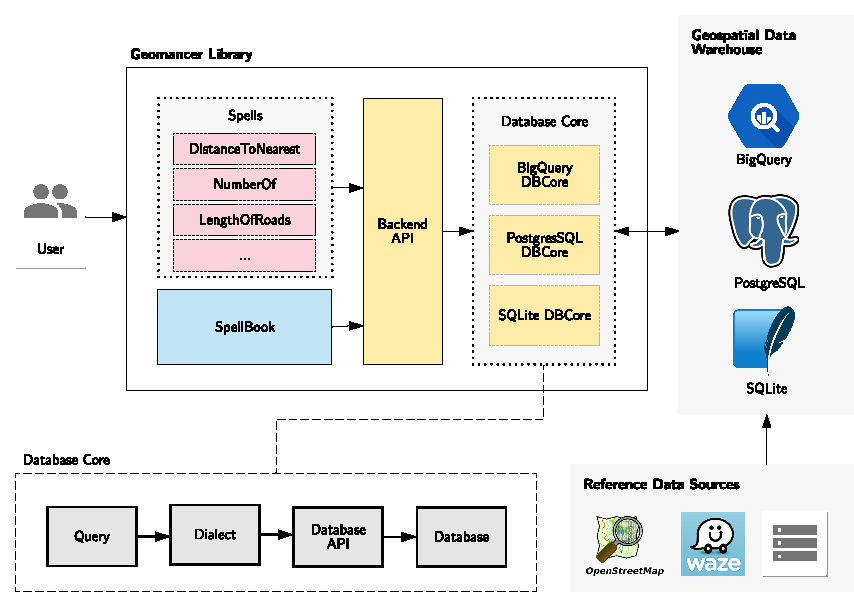
\includegraphics[width=0.85\linewidth]{architecture.pdf}
    \end{center}
  \caption{
    Architecture of the Geomancer framework. The user defines feature functions
    $\mathcal{F}$  (Spells or SpellBook) via a Python library, which are then
    executed by the DBCore as query dialects at runtime. These function-calls
    then interact with a data warehouse to fetch and store the extracted
    features. As of now, Geomancer supports BigQuery, PostgreSQL, and SQLite
    for storage with OpenStreetMap (OSM) and Waze as an external data source. 
    }

  \label{fig:architecture}
\end{figure}

\paragraph{Concepts}
The fundamental unit in Geomancer is a logical feature \cite{smith2017ballet}
called a \textit{Spell}. It maps a coordinate into a vector of feature values,
$f_{j}^{\mathcal{D}} : \mathcal{V}^{2} \rightarrow \mathbb{R}^{q_j}$, where
$\mathcal{V}$ is the set of feasible coordinates (latitude and longitude in
EPSG:4326 \cite{WGS84EPS46:online}) and $q_{j}$ is the dimensionality of the $j$th feature vector. A
collection of spells, i.e., a \textit{SpellBook}, is then defined as a set of
feature functions $\mathcal{F}^{\mathcal{D}} = \{f_j \vert j = 1 \dots m\}$. 

Geomancer allows users to define feature transforms $F^{\mathcal{D}}$, and
apply these functions to a dataset containing spatial coordinates
$\mathcal{D}^{\prime}$. The result is a feature matrix $X^{\mathcal{D}^\prime}$
\cite{smith2017ballet} that can be used for downstream machine learning tasks: 

\begin{equation}
    X^{\mathcal{D}^\prime} = 
    \mathcal{F}^{\mathcal{D}}(\mathcal{D}^\prime) = 
    (f_{1}^{\mathcal{D}}(\mathcal{D}^\prime), \dots,
    f_{m}^{\mathcal{D}}(\mathcal{D}^\prime))
\end{equation}

\paragraph{System Design} There are three main components in the Geomancer
framework: a Python library client, a data warehouse server, and an external
data source (Figure \ref{fig:architecture}). 

\begin{itemize}
    \item \textit{Python library client} The \texttt{geomancer} library
        \footnote{\url{https://pypi.org/projects/geomancer}} serves as the
        framework's user-interface. Users can define feature functions
        (Spells or SpellBooks), export/read SpellBooks, and apply transforms to
        any given spatial dataset. Creating new features is done via the
        factory design pattern whereas the SpellBook mechanism is accomplished
        using the builder pattern \cite{gamma1995design}.
    \item \textit{Data warehouse server} The data warehouse provides the
        storage and compute capacity in the framework. The library client can
        connect to multiple databases at the same time, and can handle both
        online transactional (OLTP) or analytical (OLAP) processing workloads.
        The extracted features can be stored inside the warehouse or exported
        as a dataframe for immediate consumption.
    \item \textit{External data source} An external data source is loaded
        inside the warehouse as basis for feature engineering. For example, if
        we want to obtain the number of malls within a 1.5-km radius, we should
        have some knowledge of all mall locations within the area in question.
        Fortunately, open datasets such as OpenStreetMap (OSM) \cite{osm2017}
        exists to give such information. Usually, we create
        Extract-Transform-Load (ETL) pipelines to deliver timely, rich, and
        accurate data from external sources. 
\end{itemize}

\section{Usage}

In practice, Geomancer enables researchers to (1) define geospatial features
for extraction, (2) connect to various data warehouses, and (3) replicate and
version features.  The following sections will demonstrate how this can be done
in the framework.

\paragraph{Feature functions for geospatial feature engineering}
 A \texttt{Spell} provides a declarative interface to define logical features
 \cite{smith2017ballet}. They can be \texttt{cast}ed to a set of coordinates
 after instantiation.  For example, if we wish to get the distance to the
 nearest embassy given a sample of coordinates, we write the following:

\begin{lstlisting}[language=Python]
from geomancer.spells import DistanceToNearest
from tests.conftest import sample_points

# Load a sample of points as a DataFrame
df = sample_points()

# Define a spell
spell = DistanceToNearest("embassy",
                          source_table="ph_osm.gis_osm_pois_free_1",
                          dburl="bigquery://geospatial",
                          feature_name="dist_embassy")

# Cast the spell
df_with_features = spell.cast(df)
\end{lstlisting}

\paragraph{Connect to various data warehouses}
Geomancer can establish a connection to any warehouse by providing a valid
database URL. In practice, this feature has been helpful when engineering
features across tables from different locations (e.g., OSM dataset is stored in
BigQuery, traffic dataset in PostGIS, etc.). So far, Geomancer supports the
following database backends:

\begin{itemize}
    \item BigQuery, an analytics data warehouse from the Google Cloud
        Platform \cite{google2012bigquery, melnik2010dremel}.
    \item PostGIS, a geospatial extension for PostgreSQL
        \cite{stonebraker1987postgres, stonebraker1986design}.
    \item SpatiaLite, a geospatial extension for SQLite \cite{bhosale2015sqlite,
        spatialite}.
\end{itemize}

\paragraph{Save and share feature functions}
Features can be grouped together to form a \texttt{SpellBook}, allowing us to
cast multiple \texttt{Spells} at once. In addition, \texttt{SpellBooks} can be
exported into a JSON file with various metadata (e.g., author, description,
etc.) regarding the feature collection:

\begin{lstlisting}[language=Python]
from geomancer.spells import DistanceToNearest, NumberOf
from geomancer.spellbook import SpellBook

# Create a spellbook
my_spellbook = SpellBook(
          spells=[
              DistanceToNearest("primary",
                                 dburl="bigquery://geospatial",
                                 source_table="ph_osm.gis_osm_roads_free_1",
                                 feature_name="dist_primary"),
              NumberOf("supermarket"
                        dburl="bigquery://geospatial",
                        source_table="geospatial.ph_osm.gis_osm_pois_free_1",
                        feature_name="num_supermarkets"),
          ])

# Export SpellBook into a file
my_spellbook.author = "Juan dela Cruz"
my_spellbook.description = "Good Features for Economic Indicators"
my_spellbook.to_json("my_features.json")
\end{lstlisting}

Once a \texttt{SpellBook} is exported to a file, it can be version-controlled,
shared, and reused to other datasets. In the demonstration below, the
\texttt{Spells} in the exported SpellBook, \texttt{my\_features.json}, will be
casted on a new set of points:

\begin{lstlisting}[language=Python]
from geomancer.spellbook import SpellBook
from test.conftest import sample_points_new

exported_spellbook = SpellBook.read_json("my_features.json")
df = sample_points_new() # load your own data

# Cast someone's Spells into your own data
df_with_features = exported_spellbook.cast(df)
\end{lstlisting}

\section{Case study: property value estimation in Singapore}

% Put an introduction spiel

We used Geomancer to predict residential prices per square foot in Singapore. 
The raw data was acquired from the Urban Redevelopment Authority's
open listing of apartment and condominium sales in the last
four years \cite{ura2019property}. We used this information to compile a
dataset containing the locations and unit price per square foot for over $50,000$
transactions.

% Talk about the dataset in mathematical notation
Thus, we are given a raw dataset $\mathcal{D}^{\prime} = \left\{\mathcal{V},
\mathcal{Y}\right\}$, where $\mathcal{V}$ is the property's spatial coordinate
in EPSG:4326, and $\mathcal{Y} \in \mathbb{R}$ is the unit price per square
foot. We then used Geomancer, coupled with OSM data, to define logical features
$\mathcal{F}^{\mathcal{D}}$ such as the number of restaurants within 3-km,
distance to the nearest bus stop, or distance to the nearest nightclub. This
resulted to a feature matrix $X^{\mathcal{D}}$ that will be used for model
training. 

% How many features were created? 
% Maybe you can check the dataset in BQ, it should be there

% Talk about how you trained the model. What kind of model was used?
% Check if there are any colab notebooks there

% Some interesting insights and results
% It might be important to turn the images into something "academic-y"

% Further applications


\section{Conclusion}

In this paper, we introduced Geomancer, an open-source framework to perform
geospatial feature engineering at scale. We described the Spell, a logical
feature that serves as the basic building-block of the framework. Then, we
showed how it integrates with the overall architecture and demonstrated how it
can be used through the Python client library. Lastly, we provided a sample
production use-case of Geomancer for predicting residential prices per square
foot in Singapore. Using only Geomancer-based features and OpenStreetMap data,
we were able to achieve $86\%$ accuracy with an error margin of SGD 100. 

For future research, we plan to evaluate user-efficiency and system robustness
in more detail. Finally, we also hope to expand the number of database
connections (e.g. Amazon Athena, Redshift, etc.) and primitive features to
accommodate different cloud providers and other advanced use-cases.

% acknowledgments section
\subsubsection*{Acknowledgments}

This work was supported by the UNICEF Innovation Fund. We would like to thank
our mentors for the insightful discussions and valuable guidance. 
 
\bibliographystyle{unsrt}

\small
\bibliography{bibliography}

\end{document}
